\documentclass{article}
\usepackage[utf8]{inputenc}
\usepackage{hyperref}
\usepackage{fancyhdr}
\usepackage{lipsum} 
\usepackage{lastpage} 
\usepackage{graphicx}
\usepackage{ifthen} 
\pagestyle{fancy}
\fancyhf{} 

\fancyfoot[R]{%
  \ifthenelse{\value{page}=6}{%
    \href{https://doi.org/10.2307/2331394}{Kahle, K.M. and Walkling, R.A. (1996). \textit{The Impact of Industry Classifications on Financial Research. The Journal of Financial and Quantitative Analysis}, 31(3), p.309.}%
  }{}%
}

\title{Replicate several portfolios in Ken French’s Data Library}
\author{}
\date{}

\begin{document}

\maketitle

\section*{Introduction}

The pioneering work of Fama and French have significantly influenced empirical asset pricing through their development of factor models. These models, which articulate the returns to the market factor (Rm-Rf), the size factor (SMB), and the value factor (HML), have been instrumental in academic and practical finance for over three decades. The Fama-French Data Library, that emerged from their seminal paper \textit{Common Risk Factors in the Returns on Stocks and Bonds} (1993), has evolved to become an indispensable asset for researchers and practitioners alike. This library not only facilitates access to the critical stock factors (Mkt, SMB, HML) but also underscores the dynamic nature of financial data and the continual refinement of asset pricing models.

Our project is motivated by the process of updating and refining the inputs and methodologies that underpin the Fama-French factor models. Fama and French's meticulous approach to data corrections and rule changes, as described in their recent work in \textit{Production of U.S. Rm-Rf, SMB, and HML in the Fama-French Data Library} (2023), underscores the complexity and the necessity of maintaining the highest accuracy in financial databases like CRSP (Center for Research in Security Prices) and Compustat. These databases, which provide the foundational data for constructing factor portfolios, undergo continual revisions to correct historical errors and adapt to evolving accounting standards and market realities. The adjustments made to account for such corrections directly impact the computed returns of Rm-Rf, SMB, and HML, thereby affecting the reliability and validity of empirical asset pricing research.

This project aims to replicate the univariate sorts on size, earnings/price (E/P), cashflow/price (CF/P), and dividend yield (D/P), as well as the sorts on operating profitability and investment, using unaggregated CRSP and Compustat data. In doing so, we confront the challenges of accurately linking and processing vast datasets, calculating breakpoints, and sorting stocks into portfolios that reflect the original methodologies of Fama and French. 

\section*{Data Sources}

Our replication is built upon two primary data sources: CRSP and Compustat. CRSP provided stock prices, returns, and share outstanding data, critical for calculating market equity (ME) and returns over time. Compustat offered comprehensive accounting data, including earnings, cash flows, and dividends, necessary for computing E/P, CF/P, and D/P ratios. One of the challenges in utilizing these databases was ensuring accurate linkage between CRSP and Compustat data for each stock. As a result, we employed a combination of CRSP’s PERMNO and Compustat’s GVKEY identifiers, leveraging the CRSP/Compustat Merged Database when possible to minimize mismatches. 

\section*{Methodology}

This section outlines the methodologies employed in replicating the portfolios based on Fama and French's framework, focusing on Earnings/Price (E/P), Cashflow/Price (CF/P), and the intersection of Size and Operating Profitability.

\subsection*{Portfolios Formed on Earnings/Price (E/P)}

\subsubsection*{Construction}

Portfolios were formed at the end of each June, utilizing NYSE breakpoints for sorting. The earnings considered were the total earnings before extraordinary items for the last fiscal year ending in $t-1$. The market equity (ME), defined as the product of price and shares outstanding at the end of December of $t-1$, served as the price denominator.

\subsubsection*{Portfolio Categories}

\begin{itemize}
    \item \textbf{Negative Earnings:} Firms with earnings less than zero were allocated to a distinct "Earnings < 0" portfolio.
    \item \textbf{Percentile Sorts:} The remaining firms were sorted into bottom 30\%, middle 40\%, and top 30\% portfolios based on their E/P ratios, in addition to being classified into quintiles and deciles.
\end{itemize}

\subsubsection*{Data Coverage}

The methodology was applied to all stocks listed on the NYSE, AMEX, and NASDAQ that met the data availability criteria for ME and earnings before extraordinary items from December of $t-1$ and June of $t$, spanning from July 1951 to January 2024 for monthly returns, and from 1952 to 2021 for annual returns.

\subsection*{Portfolios Formed on Cashflow/Price (CF/P)}

\subsubsection*{Construction}

Similar to E/P portfolios, CF/P portfolios were constructed at the end of each June using NYSE breakpoints. The cashflow measure included earnings before extraordinary items, equity's share of depreciation, and, if available, deferred taxes for the last fiscal year ending in $t-1$.

\subsubsection*{Portfolio Categories}

\begin{itemize}
    \item \textbf{Negative Cashflow:} Firms with a negative cashflow were allocated to a "Cashflow < 0" portfolio.
    \item \textbf{Percentile Sorts:} Other firms were sorted into bottom 30\%, middle 40\%, and top 30\% portfolios based on CF/P ratios, alongside quintile and decile classifications.
\end{itemize}

\subsubsection*{Data Coverage}

The analysis included stocks from the NYSE, AMEX, and NASDAQ with available ME for December of $t-1$ and June of $t$, and cashflow data for the calendar year $t-1$, covering annual returns from 1952 to 2021.

\subsection*{Portfolios Formed on Size and Operating Profitability}

\subsubsection*{Construction}

Portfolios were constructed at the end of each June, based on the intersections of 5 portfolios formed on operating profitability (OP) and 5 on investment (Inv). OP was calculated as annual revenues minus cost of goods sold, interest expense, and selling, general, and administrative expenses, divided by book equity for the last fiscal year ending in $t-1$. Investment was measured as the change in total assets from the fiscal year ending in $t-2$ to $t-1$, divided by total assets for $t-2$.

\subsubsection*{Portfolio Categories}

The construction resulted in 25 portfolios formed from the intersections of quintile ranks for OP and Inv, utilizing NYSE quintiles for breakpoints.

\subsubsection*{Data Coverage}

The portfolios included all NYSE, AMEX, and NASDAQ stocks with (positive) book equity for $t-1$, total assets data for $t-2$ and $t-1$, non-missing revenues data for $t-1$, and at least one non-missing data point among cost of goods sold, selling, general, and administrative expenses, or interest expense for $t-1$, covering the period from July 1963 to January 2024 for monthly returns, and 1964 to 2023 for annual returns.

\section*{Results}

This section presents the results of our replication effort, including graphical representations of the portfolios' performance and tabulated data for clearer insights into the analysis.

\subsection*{Graphical Analysis}

Figures \ref{fig:graph1} and \ref{fig:graph2} show the performance trends of the portfolios formed on Earnings/Price (E/P) and Cashflow/Price (CF/P), respectively, across different time frames.

\begin{figure}[ht]
\centering
\rule{0.8\textwidth}{0.4\textwidth} % Placeholder for graph 1
\caption{E/P Portfolio Performance Over Time}
\label{fig:graph1}
\end{figure}

\begin{figure}[ht]
\centering
\rule{0.8\textwidth}{0.4\textwidth} % Placeholder for graph 2
\caption{CF/P Portfolio Performance Over Time}
\label{fig:graph2}
\end{figure}

\subsection*{Portfolio Performance Tables}

Tables \ref{tab:ep_performance} and \ref{tab:cfp_performance} provide a detailed breakdown of the annual and monthly returns of portfolios formed on E/P and CF/P ratios.

\begin{table}[ht]
\centering
\begin{tabular}{l|l|l}
Year & E/P Portfolio Return & Benchmark Return \\
\hline
2020 & X\% & Y\% \\
2021 & X\% & Y\% \\
\end{tabular}
\caption{Annual Returns of E/P Portfolios Compared to Benchmark}
\label{tab:ep_performance}
\end{table}

\begin{table}[ht]
\centering
\begin{tabular}{l|l|l}
Year & CF/P Portfolio Return & Benchmark Return \\
\hline
2020 & X\% & Y\% \\
2021 & X\% & Y\% \\
\end{tabular}
\caption{Annual Returns of CF/P Portfolios Compared to Benchmark}
\label{tab:cfp_performance}
\end{table}


\begin{figure}[ht]
  \centering
  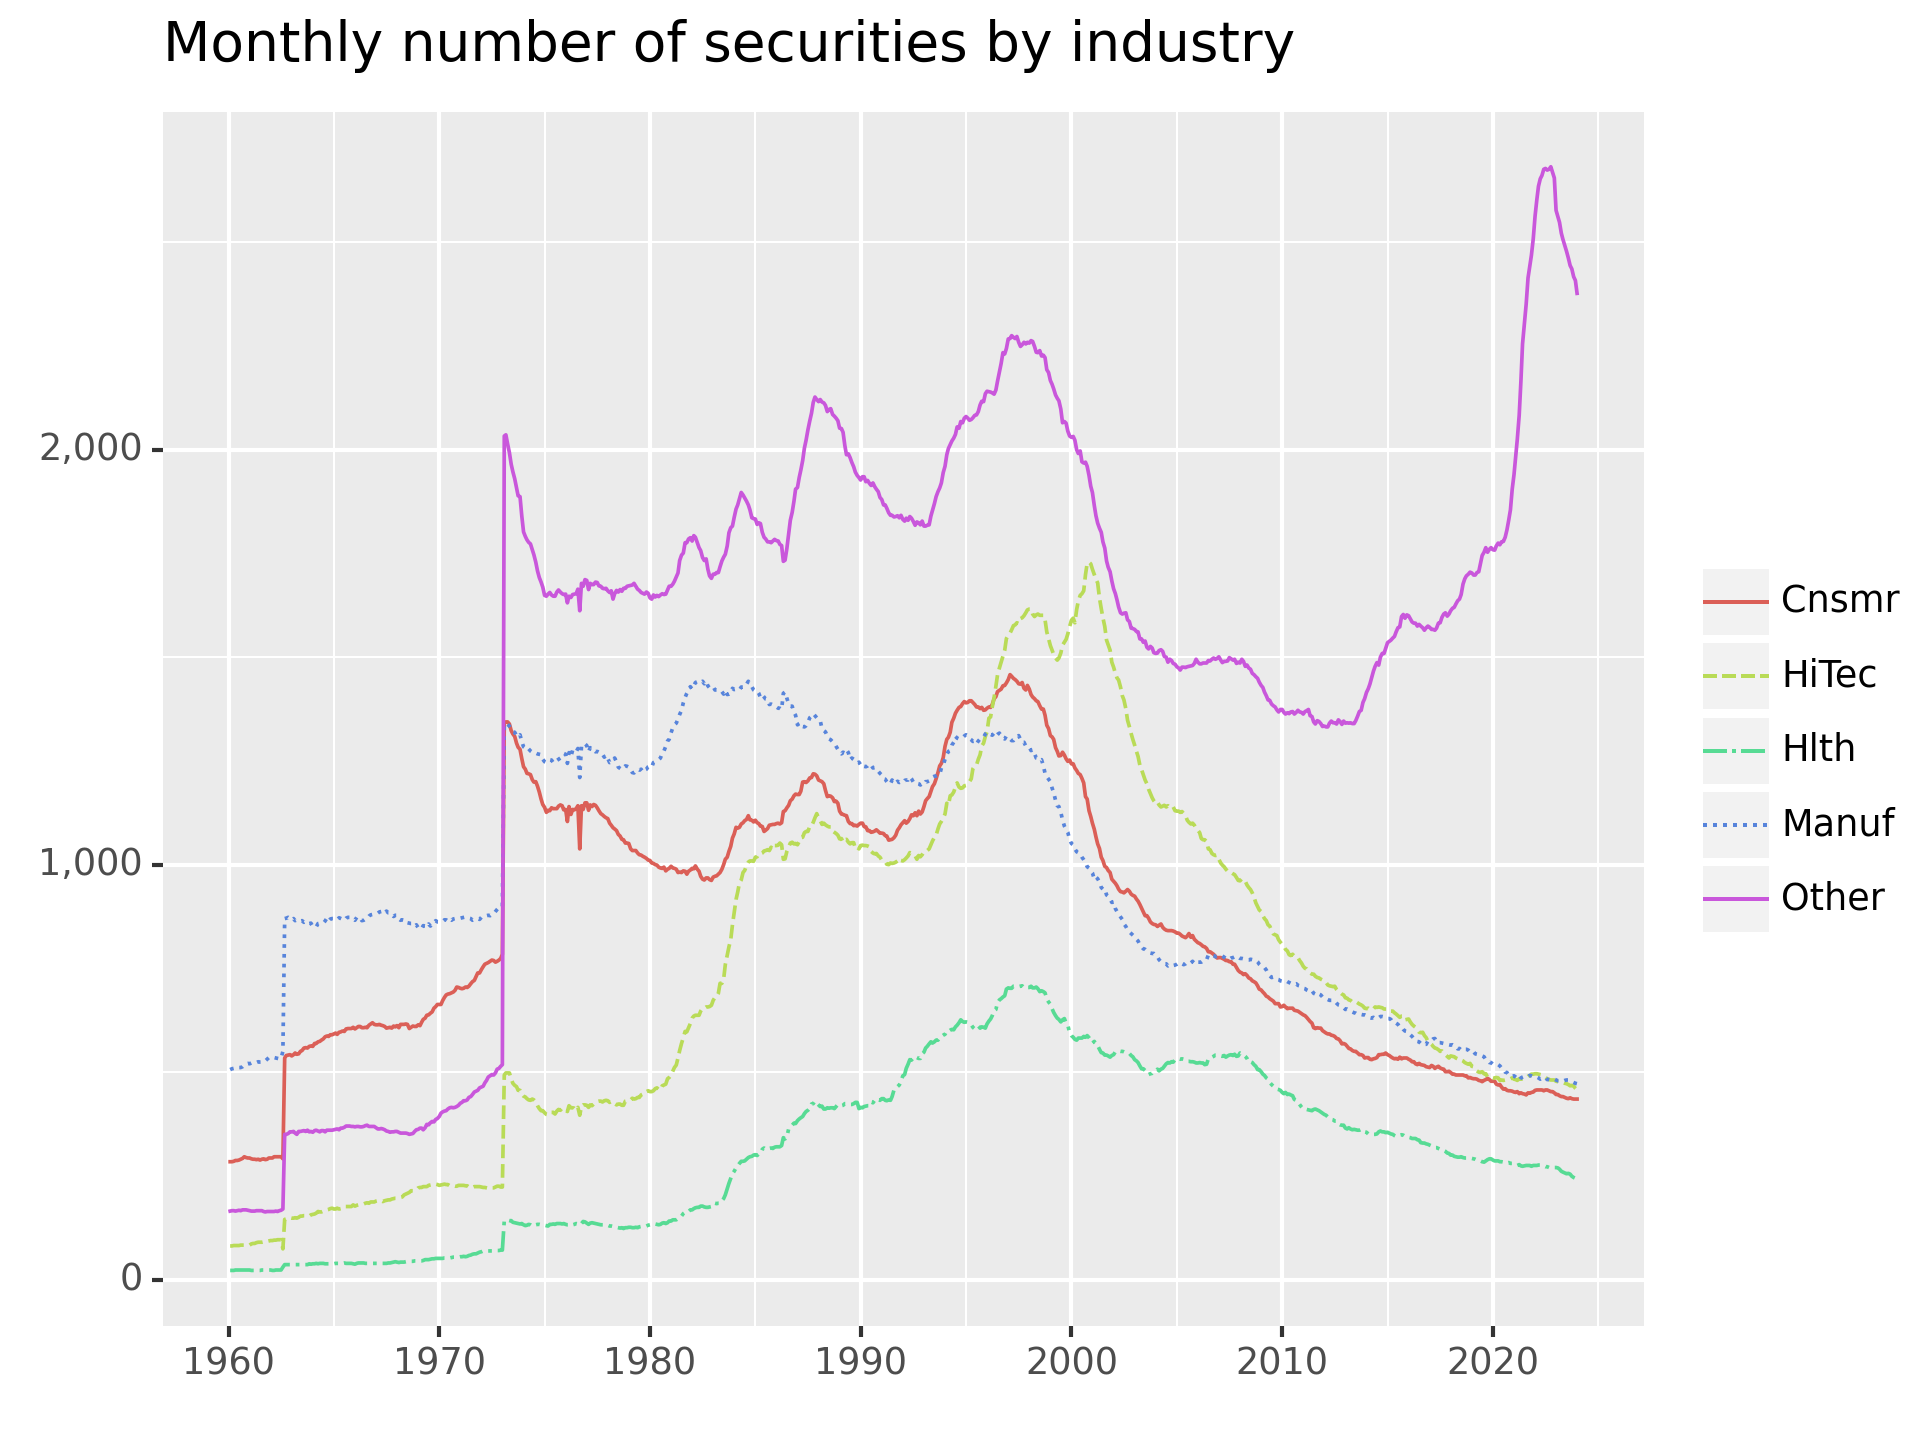
\includegraphics[width=0.8\textwidth]{output/sec_per_ind_5.png}
  \caption{A caption for the image.}
  \label{fig:my_label}
\end{figure}



\subsection*{Discussion}

[Here we can insert discussion about trends, comparisons to benchmarks, and any anomalies or significant findings observed in the data.]


\section*{Challenges in Replication}

The replication presented technical and methodological challenges that impacted our ability to precisely mirror their original findings, specifically the calculation of breakpoints and the sorting of stocks into portfolios.

\subsection*{Methodological Interpretation}

Despite rigorous documentation, practical replication efforts often encounter challenges in interpreting and applying specific methodological nuances, especially regarding the treatment of outliers or the handling of missing data. These could inadvertently lead to variations in the calculated breakpoints, impacting the composition of the resulting portfolios.

\subsection*{Portfolio Sorting Intricacies}

\subsubsection*{Conditional Sorting and Intersection}

A notable challenge in portfolio sorting was managing the conditional sorting criteria and the intersection of various metrics that is highly sensitive to the accurate calculation of each underlying portfolio. Discrepancies in any of these calculations can cascade through the sorting process, affecting the final portfolio composition.

\subsection*{Final Output and Calculation Breakdown}

A significant obstacle we faced in our replication was the challenge associated with the verification of the final output due to the absence of intermediary computational results. This limitation becomes particularly pronounced when attempting to identify and correct discrepancies, as the process lacks transparency without access to detailed breakdowns of each calculation step. Such a situation makes it difficult to pinpoint errors, requiring, each time, a meticulous review of the entire computational procedure to ensure accuracy.

\subsection*{Data Availability and SIC Code Challenges}

Furthermore, the replication was compounded by missing data points within the code, which made the construction of accurate functions and the execution of complex calculations more difficult. The evolution and changes in Standard Industrial Classification (SIC) codes over an extensive period (80+ years) presented another layer of complexity. 

The discrepancies between the CRSP and Compustat databases regarding a range of values added inconsistencies that significantly impacted the fidelity of replication efforts, as they may introduce variances in the data set that are not present in the original studies. The study on the stability and reliability of financial variables over time by Kahle, K.M. and Walkling, R.A. (1996) in the \textit{Journal of Financial and Quantitative Analysis}, highlights the difficulties in maintaining consistent data classifications over prolonged periods and underscores the potential for classification and data discrepancies to skew results.

\end{document}
